%\begin{noindent}
\begin{markdown}
# Kompensationsanlagen

\GrayBox{Um das Netz vor Spannungsabfällen und Verlusten zu entlasten, werden bei Verbrauchern mit **großen Blindstrombedarf** Kompensationsalnagen installiert.}

Es gibt auch **zentrale Kompensationsanlagen**, um den Blindstromeinfluss im Netz zu steuern und zu optimieren.

**Wesentliche Blindleistungsverbraucher:**

- Leuchtstofflampen
- schwach belastete Asynchronmotoren
- Antriebe mit Stromrichtern
- Freileitungen und Transformatoren

Durch die zusätzliche Blindleistung müssen die Übertragungswege größer ausgelegt werden - die Kraftwerke werden mehr ausgelastet.

Die Blindstromverluste können am Ort der Erzeugung mittels Kondensatoren teilweise kompensiert werden - die Blindleistung pendelt somit nur mehr zwischen Verbraucher und Kompensationsanlage.

\vspace{2em}

\begin{figure}[H]
    \centering
    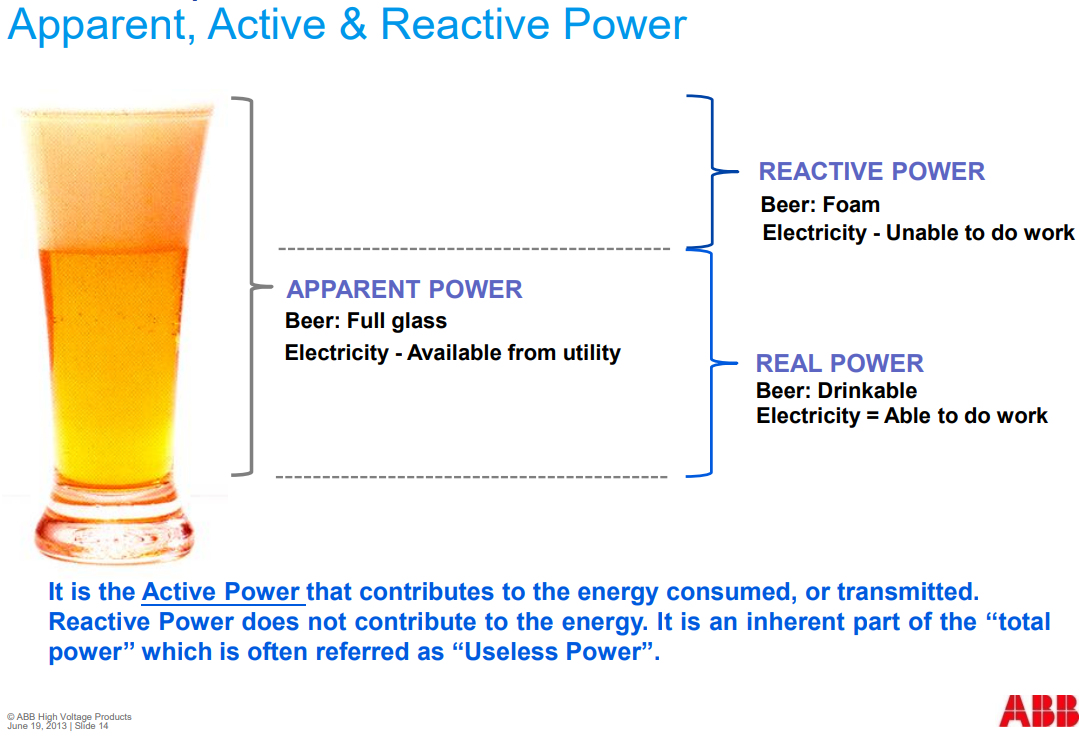
\includegraphics[width=\linewidth]{./images/11-Kompensationsanlagen/Reactive-Power-Compensation-ABB.png}
    \caption[Beispiel für Blindleistung]{Beispiel für Blindleistung}
\end{figure}

\newpage

## Gruppenkompensation

\GrayBox{Die Gruppenkompensation wird bei Verbrauchern mit gleichem Betriebsverhalten eingesetzt. (z.B.: Lichtbänder)}

\begin{wrapfigure}{r}{0.4\textwidth}
    \vspace{-1em}
    \centering
    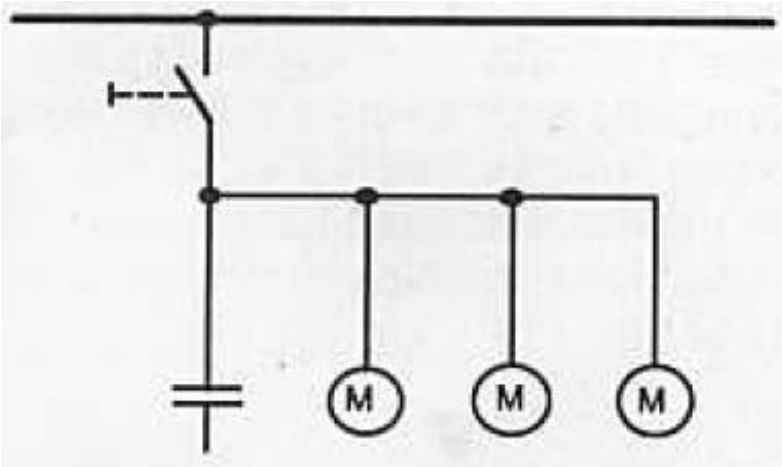
\includegraphics[width=0.8\linewidth]{./images/11-Kompensationsanlagen/Gruppenkompensation.png}
    \caption[Gruppenkompensation]{Gruppenkompensation}
\end{wrapfigure}

**Vorteile:**

- Niedrige Kosten
- Stromwärme-Verluste werden verringert
- Spannungsabfälle werden verringert

**Nachteile:** Stromkreisleitungen werden **nicht** entlastet

\vspace{4em}

## Zentralkompensation

\GrayBox{Die Zentralkompensation wird bei größeren Anlagen und bei ständig wachsender Last eingesetzt.}

**Vorteile:**

- Kondensator-Leistungen können geregelt werden (je nach Blindleistungsbedarf) 
- Nachträgliche Installationen sind möglich

**Nachteile:** Stromkreisleitungen werden **nicht** entlastet

\begin{figure}[H]
    \centering
    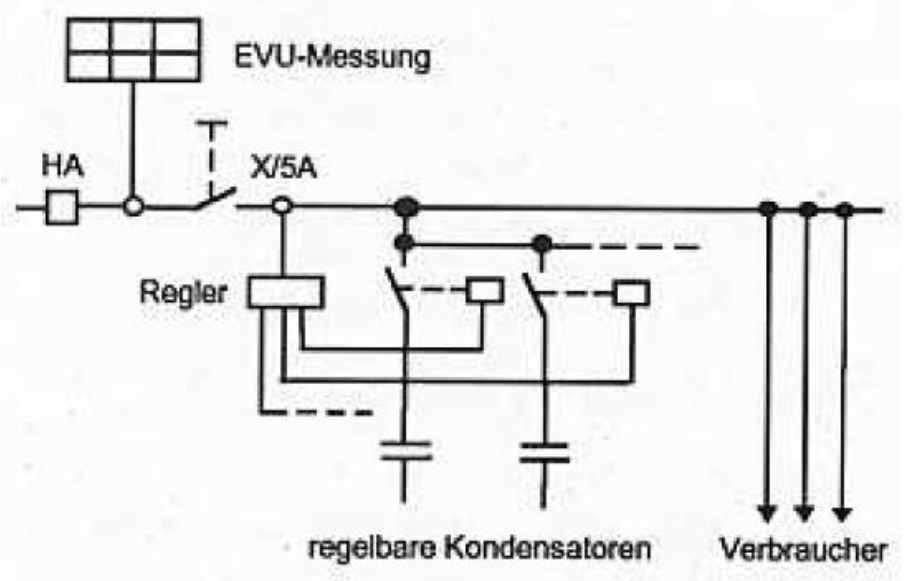
\includegraphics[width=0.5\linewidth]{./images/11-Kompensationsanlagen/Zentralkompensation.png}
    \caption[Zentralkompensation]{Zentralkompensation}
\end{figure}

## Netzrückwirkungen

- Spannungsspitzen durch die Kondensatoren
- Leistungselektronik in den Netzen benötigen Blindleistung 
- Hohe Oberschwingungsströme von Stromrichter gefährden die Kondensatoren _(Kompensationsdrosseln wären erforderlich)_

\end{markdown}